% fig_zseq_zm_ibr.tex
% TR-31: |Zm| vs alpha for IBR-fed SLG faults (k0-compensated relay)
%
% Data from run_zseq_compensation_study.py Study C:
%   IBR k=0.06: (0.20,0.079) (0.50,0.103) (0.80,0.127) (1.00,0.143)
%   IBR k=0.10: (0.20,0.077) (0.50,0.100) (0.80,0.123) (1.00,0.138)
%   IBR k=0.15: (0.20,0.074) (0.50,0.096) (0.80,0.118) (1.00,0.133)
%   IBR k=0.20: (0.20,0.071) (0.50,0.092) (0.80,0.113) (1.00,0.127)
%   SG (true):  (0.10,0.005) (0.20,0.010) (0.50,0.025) (0.80,0.040) (1.00,0.050)
%
% Key boundaries:
%   Zone 1 reach: X_R1 = 0.040 pu
%   Zone 2 reach: X_R2 = 0.060 pu
%   Zone 3 reach: X_R3 = 0.090 pu
%
% Finding: IBR Zm >> true value; only Zone 3 fires for close-in faults (alpha<~0.35)
%          Zone 1 and Zone 2 never fire for ANY IBR-fed SLG fault.

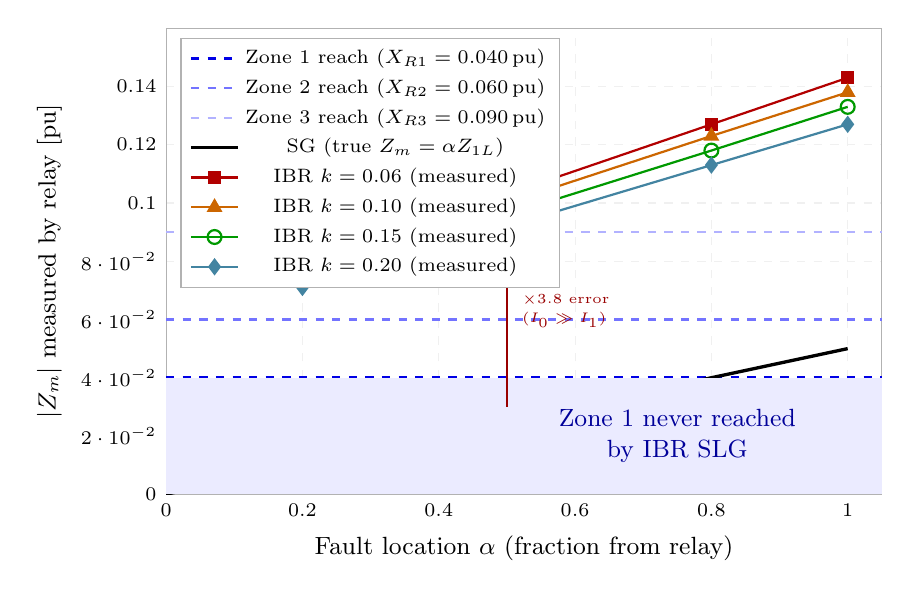
\begin{tikzpicture}
\begin{axis}[
  name         = zmibr,
  width        = 0.88\textwidth,
  height       = 7.5cm,
  xlabel       = {Fault location $\alpha$ (fraction from relay)},
  ylabel       = {$|Z_m|$ measured by relay [pu]},
  xlabel style = {font=\small},
  ylabel style = {font=\small},
  xmin=0.0, xmax=1.05,
  ymin=0.0,  ymax=0.160,
  xtick        = {0, 0.2, 0.4, 0.6, 0.8, 1.0},
  ytick        = {0, 0.02, 0.04, 0.06, 0.08, 0.10, 0.12, 0.14},
  xticklabel style={font=\scriptsize},
  yticklabel style={font=\scriptsize},
  legend style={at={(0.02,0.98)}, anchor=north west,
                font=\scriptsize, draw=gray!60, fill=white},
  grid         = major,
  grid style   = {gray!12, dashed},
  tick style   = {draw=none},
  axis line style={gray!60},
]

%% ── Zone reach lines ────────────────────────────────────────────────────────
\addplot[blue!90!black, very thick, dashed, mark=none]
  coordinates {(0,0.040) (1.05,0.040)};
\addlegendentry{Zone~1 reach ($X_{R1}=0.040$\,pu)}

\addplot[blue!55, thick, dashed, mark=none]
  coordinates {(0,0.060) (1.05,0.060)};
\addlegendentry{Zone~2 reach ($X_{R2}=0.060$\,pu)}

\addplot[blue!30, thick, dashed, mark=none]
  coordinates {(0,0.090) (1.05,0.090)};
\addlegendentry{Zone~3 reach ($X_{R3}=0.090$\,pu)}

%% ── SG true Z_m (reference) ─────────────────────────────────────────────────
\addplot[black, very thick, mark=none]
  coordinates {(0,0) (0.10,0.005) (0.20,0.010) (0.40,0.020) (0.60,0.030)
               (0.80,0.040) (1.00,0.050)};
\addlegendentry{SG (true $Z_m=\alpha Z_{1L}$)}

%% ── IBR measured Z_m (k0-compensated) ───────────────────────────────────────
\addplot[red!70!black, thick, mark=square*, mark size=2pt]
  coordinates {(0.20,0.079) (0.50,0.103) (0.80,0.127) (1.00,0.143)};
\addlegendentry{IBR $k=0.06$ (measured)}

\addplot[orange!80!black, thick, mark=triangle*, mark size=2.5pt]
  coordinates {(0.20,0.077) (0.50,0.100) (0.80,0.123) (1.00,0.138)};
\addlegendentry{IBR $k=0.10$ (measured)}

\addplot[green!60!black, thick, mark=o, mark size=2.5pt]
  coordinates {(0.20,0.074) (0.50,0.096) (0.80,0.118) (1.00,0.133)};
\addlegendentry{IBR $k=0.15$ (measured)}

\addplot[cyan!60!black, thick, mark=diamond*, mark size=2.5pt]
  coordinates {(0.20,0.071) (0.50,0.092) (0.80,0.113) (1.00,0.127)};
\addlegendentry{IBR $k=0.20$ (measured)}

%% ── Shaded "Zone 1 region" ──────────────────────────────────────────────────
\addplot[fill=blue!8, draw=none]
  coordinates {(0,0) (1.05,0) (1.05,0.040) (0,0.040)};

%% ── Annotation: Zone 1 never reached ────────────────────────────────────────
\node[font=\small, blue!60!black, align=center]
  at (axis cs:0.75, 0.020)
  {Zone 1 never reached\\by IBR SLG};

%% ── Annotation: Zone 3 window ───────────────────────────────────────────────
\node[draw=orange!60, fill=orange!8, rounded corners=2pt,
      font=\tiny, align=left, inner sep=3pt]
  at (axis cs:0.20, 0.118)
  {Zone~3 fires for $\alpha \lesssim 0.35$\\
   (close-in SLG only)};

%% ── Arrow showing large over-estimation ─────────────────────────────────────
\draw[->, thick, red!60!black]
  (axis cs:0.50, 0.030) -- (axis cs:0.50, 0.096);
\node[right=2pt, font=\tiny, red!60!black, align=left] at (axis cs:0.50, 0.063)
  {$\times3.8$ error\\[1pt]($I_0\gg I_1$)};

\end{axis}
\end{tikzpicture}
